\documentclass{scrartcl}
\usepackage{amsmath}
\usepackage[ngerman]{babel}
\usepackage{amsfonts}
\usepackage{amssymb}
\usepackage{graphicx}
\usepackage{figsize}
\usepackage{float}
\usepackage{geometry}
\geometry{verbose,tmargin=2.5cm,bmargin=2.5cm,lmargin=2.5cm,rmargin=2.5cm}
\usepackage[format=plain,font=small,labelfont=bf]{caption}
\usepackage[OT2,T1]{fontenc}
\DeclareSymbolFont{cyrletters}{OT2}{wncyr}{m}{n}
\DeclareMathSymbol{\Sha}{\mathalpha}{cyrletters}{"58}
\selectlanguage{ngerman}
\begin{document}

\thispagestyle{empty}
\vspace*{\fill}
\begin{center}
	\Huge
	\textbf{Universität zu Köln}\\
	\LARGE
	\textbf{Institut für Astrophysik}\\ 
	\vspace{2cm}
	\textbf{Versuchsprotokoll}\\
	\vspace{0.5cm}
	\large
	\textbf{B1.3: Bestimmung der Elementarladung nach Millikan}\\
	\normalsize
	\vspace{2cm}
	\begin{tabular}{r l}
		Autoren: 	& Jesco Talies$^1$\\
					& Timon Danowski$^2$\\
		Durchgefuehrt am:	& 19.04.2021\\
		Betreuer:	& Marius Hermanns
	\end{tabular}
\end{center}
\vfill\footnotesize
$^1$ jtalies@smail.uni-koeln.de, Matrikel-Nr.: 7348338\\
$^2$ tdanowsk@smail.uni-koeln.de, Matrikel-Nr.: 7348629\\
\normalsize

\newpage 
\thispagestyle{empty}
\tableofcontents
\clearpage
\setcounter{page}{1}

\section{Versuchsvorbereitung}
	\subsection{Motivation}
		Bereits in den 1890er Jahren wurden erstmals versuche zu Elektronen durchgeführt, damals
		beschränkte sich das wissen zunächst auf die interaktion zwischen Elektronenstrahlen und elektrischen-,magnetischen feldern.
		Damals experimentell ergründet anhand von kathodenstrahlen durch J.J. Thompson. Er versuchte die erste quantitative aussage über einen
		solchen kathodenstrahl zu treffen, idem er dessen bewegung in einem Magnetfeld beobachtete. Bereits damals
		wusste er das die Lorentzkraft die einzig notwendige Zentripetalkraft für eine Kreissbahn sein musste.
		Damit begründete er zunächst die Naturkonstante $\frac{e}{m_e}$ als Verhältnis von ladung zu masse.
		Im rahmen der genaueren bestimmung der Elementarladung entwickelte Harvey Fletcher angeregt von Robert Millikan im Rahmen
		seiner Doktorarbeit den hier beschriebenen und durchgeführten versuch. Durch diesen war die bestimmung
		der Elementarladung deutlich präzieser als mit vorherigen experimenten zu selbiger.
		Für die Messungen von Harvey Fletcher erhielt Robert Millikan 1923 den Nobelpreis.  
		\\
		Um das konzept einer quantisierten, bzw. der kleinsten quantisierbaren ladung genauer
		zu ergründen bietet sich im rahmen eines Praktikums kaum ein versuch besser an als eben dieser.
		Er vereint Gravitation, Elektrostatik, Reibung und Auftrieb als folge der Gravitation um durch
		geladene mikroskopische öltröpfchen und deren bewegung zwischen kondensatorplatten um durch das
		herschende kräfteverhältnis die ladung der tröpfchen präziese zu bestimmen.
		\\
		Im versuch werden wir analog zu Harvey Fletcher die Steig- und Fallzeiten verschieden geladener
		Öltröpchen messen und durch eine vorgegebene kondensatorspannung die Ladung der Tröpfchen erhalten.
		Ziel dieser messung ist die reproduktion des ursprünglichen versuchs und die quantisierung der Elementarladung,
		unter betrachtung des physikalischen systems.
	\subsection{Die Elementarladung}
		Die Elementarladung, der Zentrale kern dieses Versuchs, ist die kleinst mögliche frei existierende Ladung. Ihr Wert beträgt
			\begin{equation}
				e = 1,602 176 634 * 10^{-19} C
			\end{equation}
		Sie wird häufig verwendet um die Ladung eines einzelnen Elektrons bzw. Protons zu beschreiben. Ladungen
		freier teilchen teilchen oder gar makroskopischen systemen lässt sich stehts als ein ganzzahliges vielfaches
		dieser ladung schreiben. Die erkenntniss über eben diese additive bzw. quantitative natur wird Robert Millikan zugeschrieben.

	\subsection{Kräfte im Versuch}
		In diesem Versuch befinden sich Öltröpchen in einem Plattenkondensator unter dem Einfluss verschiedener Kräfte.
		In abbildung \ref{forces} sind diese einmal grob dargestellt. Dabei kennzeichnen die Fettgedruckten buchsteaben eine
		Vektorielle größe.
		\begin{figure}[H]
			\centering
			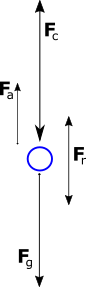
\includegraphics[width=0.1\textwidth]{kräfte.png} 
			\caption{Darstellung der Kräfte auf ein geladenes öltröpfchen (blau)}
			\label{forces}
		\end{figure}

		\subsubsection{Coulomb Kraft [ $\vec{F_c}$ ]}
			Die domininierende Kraft in diesem Versuch ist die Coulomb Kraft. Sie definiert die Kraft auf eine Punktladung oder ein
			geladenes Makroskopisches Objekt in anwesenheit eines Elektrischen feldes. In diesem Fall wird das Elektrische Feld
			durch den Plattenkondensator erzeugt und übt eine Kraft auf die Geladenen Öltröpfchen aus. Diese Kraft ist im \ref{forces}
			gekenzeichnet durch $\vec{F_c}$ und lässt sich beschreiben durch
			\begin{equation}
				\vec{F_c} = Q \cdot \frac{\pm U}{d} \vec{e}_z
			\end{equation}
			wobei Q die Ladung des Objektes ist, U die Spannung zwischen den Kondensatorplatten und d der Abstand der Kondensatorplatten ist.
			Die Richtung der resultierenden Kraft hängt dabei von der Polarisierung des Kondensators ab. Polt man diesen über den Kommutatorschalter \ref{kommutator}
			um, so ändert sich auch die Richtung der wirkenden kraft. Sie ändert sich auch mit der Ladung des Objektes selber,
			diese lässt sich jedoch in diesem aufbau nicht kontrollieren.	
		
			\subsubsection{Gravitationskraft [ $\vec{F_g}$ ]}
			Die nächst größte Kraft ist hier die Gravitationskraft, sie beschreibt die Wirkung eines Massereichen Objektes,
			hier der Erde, auf eine zweite Masse. Streng genommen beschreibt sie auch die Anziehende wirkung zwischen kleineren
			massen, jedoch sind diese in anwesenheit einer weitaus massereicheren objektes zu vernachlässigen.
			Im gravitationsfeld der Erde lässt sich die Kraft auf die die Öltröpchen über
			\begin{equation}
				\vec{F_g} = m\vec{g}
			\end{equation}
			wobei m die Masse des Objektes (hier das Öltröpchen) und g die lokale Erdbeschleunigung mit $g = 9,80665 \frac{m}{s^2}$ ist ($\vec{g} = g \cdot -\vec{e}_z$) beschreiben.
			sie wirkt stehts in richtung der Erdoberfläche und ist unabhängig von der Ladung der Tröpfchen. Sie wirkt entweder
			der Coulombkraft entgegen oder Addiert sich zu ihr, daraus folgt auch das die Coulombkraft dominieren muss damit man den
			steigvorgang der Tröpfchen beobachten kann.
		
			\subsubsection{Auftriebskraft [ $\vec{F_a}$ ]}
			Die Auftriebskraft ist eine der Gravitationskraft entgegenwirkende größe, sie beschreibt die scheinbare
			massenabnahme eines Objekts durch die Verdrängung des umschließenden Mediums. Sie wirkt daher, das der
			druck auf ein umschlossenes Object mit der Eintauchtiefe zunimmt und für makroskopische objekte somit
			nicht als konstant angenommen werden kann. Sie hängt ab von der Dichte des umschließenden Mediums, bzw. des davon abhängigen Drucks,
			dem Volumen des Objekts und der Gravitationsbeschleunigung.
			Ein Tröpchen mit dem Radius r erfährt in der Luft unter der Erdbeschleunigung eine Auftriebskraft:
			\begin{equation}
				\vec{F_a} = - \rho_{Luft} \frac{4}{3} \pi r^3 \vec{g}
			\end{equation}
			mit $\rho_{Luft}$ als Dichte der Luft. Dabei beschreibt $V=\frac{4}{3} \pi r^3$ das Volumen einer Kugel.
			Da die dichte der Luft, oder gasen im allgemeinen, im vegleich zu üblichen fluiden wie Wasser, oder flüssigkeiten im allgemeinen, an denen üblicherweise
			der begriff der Auftriebskraft demonstriert wird, ist die Auftriebskraft verschwindent gering.
		
			\subsubsection{Reibungskraft [ $\vec{F_r}$ ]}
			Reibungskräfte sind geschwindigkeitsabhängige Widerstandskräfte, die der Bewegung eines Körpers entgegenwirken.
			Man unterscheidet zwischen äußerer und innerer Reibung.
			Reibung entsteht im allgemeinen durch energieaustausch eines Bewegten Objektes mit seiner Umgebung,
			so gibt ein Festkörper im falle von äusserer Reibung durch seine Kontaktfläche mit anderen Festkörpern
			einen Teil seiner Bewegungsenergie an diese ab, die daraus resultierende negative beschleunigung wirkt
			der ursprünglichen bewegungsrichtung entgegen und lässt sich in verbindung mit der masse des objektes als
			Kraft interpretieren. Inner reibung wirkt ähnlich, hier tritt der Energieverlust durch die verformung
			benachbarter teilchen innerhalb eines Festkörpers, Flüssigkeit oder wie hier einem Gaß auf.
			Für diesen Versuch interessiert uns die innere Reibung, welche sich aus der Viskosität des Mediums ableitet.
			Die Stokes-Reibungskraft auf eine Kugel mit dem Radius r und Geschwindigkeit v, welche sich durch ein Medium der Viskosität $\eta$ bewegt ergibt sich zu
			\begin{equation}
				\vec{F_r} = -6 \pi r \eta \vec{v}
			\end{equation}
		\subsubsection{Cunningham-Korrektur}
			Wenn der Radius eines Teilchens im Bereich der mittleren freien Weglänge des umgebenden Mediums liegt, trifft das Stoke´sche Reibungsgesetz nicht mehr zu.
			Dies liegt daran, dass die Stoke´sche Reibung die äußere Reibung zwischen Öl und Luft vernachlässigt.
			Unter Verwendung der Cunningham-Korrektur ändert sich die Stoke´sche Reibung zu:
			\begin{equation}
				\vec{F}_R = -6 \pi r \eta \vec{v} \cdot (1 + A_c \frac{<l>}{r})^{-1}
			\end{equation}
			wobei $<l>$ die mittlere freie Weglänge und $A_c$ eine Konstante ist, für die wir den Wert $A_c = 1,26$ verwenden werden.
		\subsection{Herleitung der Formeln}
			Aus den wirkenden Kräften können wir uns jetzt Formeln für den Radius und die Ladung eines Öltröpchens herleiten.
			Im Kräftegleichgewicht ist die Summe aller wirkenden Kräfte gleich 0.
			Das Medium in dem sich die Tröpchen bewegen ist Luft, daher	$\rho_m  = \rho_{Luft}$ und $\rho_K = \rho_{Öl}$
			Ein Tröpchen steigt für
			\begin{equation}
				\vec{F}_C + \vec{F}_A > \vec{F}_G
			\end{equation}
			wegen der entgegenwirkenden  Reibungskraft gleichmäßig mit:
			\begin{equation}
				\vec{v}_{steig} = \frac{1}{6\pi \eta r} (Q \frac{U}{d} - \frac{4}{3}\pi r^3 -(?)g (\rho_{Öl}-\rho_{Luft})) \cdot \vec{e}_z
			\end{equation}
			Bei Umpolung der Kondensatorplatten ($\vec{F}_C + \vec{F}_A < \vec{F}_G$), ergibt sich für die Sinkgeschwindigkeit:
			\begin{equation}
				\vec{v}_{sink} = \frac{1}{6\pi \eta r} (Q \frac{U}{d} + \frac{4}{3}\pi r^3 -(?)g (\rho_{Öl}-\rho_{Luft})) \cdot \vec{e}_z
			\end{equation}

			Durch Subtraktion der beiden Gleichungen und umstellen nach r, erhält man:
			\begin{equation}
				r = \sqrt{\frac{9 \eta (v{sink} - v_steig)}{4 g (\rho_{Öl} - \rho_{Luft})}}
			\end{equation}

			Durch Addition der beiden Gleichungen, Einsetzen von 0 oben und anschließendem umstellen nach Q, erhält man:
			\begin{equation}
				Q = \frac{3 \pi d \eta r}{U} (v_{sink} + v_{steig})
				\rightarrow \frac{9}{2} \pi d \sqrt{\frac{\eta^3 (v_{sink} - v_{steig})}{g (\rho_{Öl} - \rho_{Luft})}} \frac{v_{sink} + v_{steig}}{U} 
			\end{equation}

			Mit der Cunningham Korrektur kommt man mit den selben Schritten auf den Radius:
			\begin{equation}
				r_C = \frac{A_c <l>}{2} + \sqrt{\frac{A_C <l>}{2}^2 +\frac{9 \eta (v_{sink} - v_{steig})}{4 g (\rho_{Öl} - \rho_{Luft})}}
					= \frac{A_c <l>}{2} + \sqrt{\frac{A_C <l>}{2} + r^2}
			\end{equation}
			und die Ladung:
			\begin{equation}
				Q_C = \frac{3 \pi \eta r_C d}{U} (1 + A_C \frac{<l>}{r_C})^{-1} (v_{sink} + v_{steig})
				\rightleftarrows Q \cdot \frac{r_C}{r} (1 + A_C \frac{<l>}{r_C})^{-1} 
			\end{equation}

\section{Durchführung}
	\subsection{Aufbau}
		\begin{figure}[H]
			\centering
			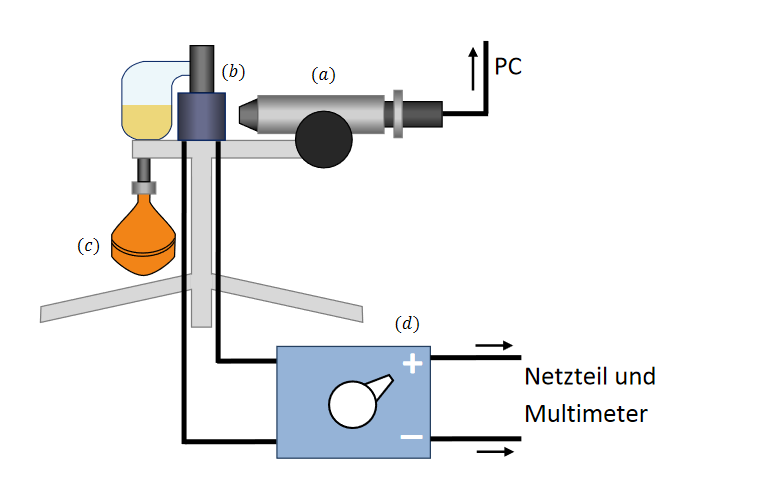
\includegraphics[width=1.0\textwidth]{Versuchsaufbau.PNG}
			\caption{Versuchsaufbau}
			\label{versuchsaufbau}
		\end{figure}
		\begin{itemize}
			\item (a) Mikroskop mit vorgeschalteter Kamera
			\item (b) Kammer mit Plattenkondensator
			\item (c) Ölstäuber mit Blasebalg
			\item (d) Kommutatorschaltung
		\end{itemize}
	\subsection{Kommutatorschalter}
		\begin{figure}[H]
			\centering
			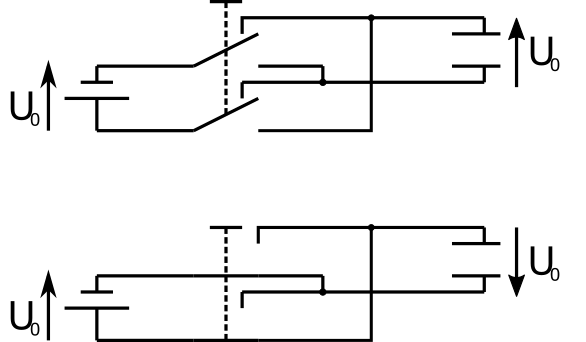
\includegraphics[width=.5\textwidth]{kommutator.png} 
			\caption{Schaltplan eines Kommutator bzw. Wechselschalters in beiden Stellungen}
			\label{Kommutator} 
		\end{figure}
		Der Kommutatorschalter oder besser Wecheslschalter wird benötigt um die Polarität des Kondensators und damit die Polarität
		und die Bewegungsrichtung der geladenen Tröpfchen zu ändern. Dazu werden die kontakte wie in \ref{Kommutator} illustriert.
		Dazu werden die Kontakte des Schalters zwischen den Polen des Kondensators gewechselt um so die Polarität desselbigen zu ändern.
	\subsection{Strahlengang}
		

	\subsection{Versuchsdurchführung}
		Zu Beginn des Versuchs müssen sowohl Mikroskop als auch Kamera kalibiriert werden. Dafür wird zunächst die
		Spannungsversorgung der Mikroskopkamera angeschaltet und dessen Addresse und Konfiguration über die 'Commen Vision Blox Management Console'
		gesucht und gespeichert um im folgenden das Bild der Kamera im Programm 'MovieInteractive 2' zu betrachten
		und die Belichtungszeit und Verstärkung der Kamera zu kalibrieren. Hierbei sollte darauf geachtet werden, dass die 
		Belichtungszeit nicht zu lang ist, da dies zu "Verschmierung" der Tropfen im Bild führt. Auch sollte 
		die Verstärkung nicht zu groß gewählt werden um das Rauschen des Hintergrunds gering zu halten. Hat man 
		eine aktzeptable Konfiguration gewählt sollte die Brennebene des Mikroskops in die Mitte des Plattenkondensators
		verschoben werden um die Tröpfchen zu filmen.
		Um die Steig- und Sinkzeit eines Tröpfchens zu messen wird zunächst der Blasebald betätigt um einige
		Öltröpchen zu zerstäuben. Anschließend wird durch wiederholtes Umpolen des Kondensator ein geladenes Tröpfchen 
		identifiziert und die Aufnahme kann über den Computer gestartet werden. Bei der Aufnahme sollten mindestens fünf
		vollständige Steig- und Sinkvorgänge aufgezeichnet werden um die Fehler in der Auswertung gering zu halten.
		Hierzu wartet man bis das Tröpfchen eine der äusseren Begrenzungen der Milimeterskala überschreitet und polt dann
		das Feld des Kondensators um und lässt es über die gegenüberliegende Begrenzung wandern.
		Dieser Prozess wird für insgesamt 20 Tröpfchen wiederholt. Es ist dabei darauf zu achten stehts
		die Brennebene des Mikroskops nach zu justieren, da die Tröpfchen durch Verwirbellung und Stöße mit 
		Luftpartikeln leicht aus der Brennebene wandern und dann nicht länger auf der Aufnahme zu sehen sind.
\section{Auswertung}
	Die Fallzeiten der oben beschriebenen Messung können anschließend durch Frameweise betrachtung der Aufnahmen
	extrahiert werden.
	Aus unseren gemessenen Steig- und Sinkzeiten ergaben sich folgende Mittelwerte und deren Fehler
	\begin{equation}
		\bar{t} = \frac{1}{n} \cdot \sum_{i=1}^n t_i
	\end{equation}
	\begin{equation}
		\Delta \bar{t} = \sqrt{\frac{1}{n\cdot(n-1)}\cdot \sum_{i=1}^n{t_i - \bar{t}}}
	\end{equation}
	mit n = Anzahl der Messwerte (hier 5) und $t_i$ = Messwert.
	Wobei 
	\begin{equation}
		t = \frac{Frame(Ende)-Frame(Start)}{Framerate}
	\end{equation}
	mit Framerate = 32,792 Bilder/s, somit ist t in Sekunden.

	Die Geschwindigkeiten ergeben sich über
	\begin{equation}
		v = \frac{s}{t}
	\end{equation}
	mit $s = (0.96 \pm 0.01) \mu m$ und ein Fehler von
	\begin{equation}
		\Delta v = v \cdot \sqrt{(\frac{\Delta s}{s})^2 + (\frac{\Delta t}{t})^2} 
	\end{equation}

	Daraus lässt sich der Radius folgendermaßen berechnen
	\begin{equation}
		r = \sqrt{\frac{9\eta \cdot (v_{sink}-v_{steig})}{4 g \cdot (\rho_{Öl}-\rho_{Luft})}}
	\end{equation}
	mit $\eta = 1.81e-5 Pa\cdot s$, $g=9.81 \frac{m}{s^2}$, $\rho_{Öl} = 1030 \frac{kg}{m^3}$, $\rho_{Luft} = 1.29 \frac{kg}{m^3}$
	und den Fehler
	\begin{equation}
		\Delta r = \frac{r}{2} \cdot \sqrt{(\frac{\Delta \eta}{\eta})^2+\frac{\Delta v_{sink}^2+\Delta v_{steig}^2}{(v_{sink}-v_{steig})^2}}
	\end{equation}
	und ebenfalls die Ladung Q
	\begin{equation}
		Q = \frac{3\pi \cdot d\eta}{U} \cdot r \cdot (v_{sink}+v_{steig})
	\end{equation}
	und der Fehler
	\begin{equation}
		\Delta Q = Q \cdot \sqrt{(\frac{\Delta \eta}{\eta})^2 + (\frac{\Delta d}{d})^2+(\frac{\Delta r}{r})^2 + \frac{\Delta v_{sink}^2 + \Delta v_{steig}^2}{(v_{sink} + v_{steig})^2}}
	\end{equation}
	damit ergab sich die folgende Tabelle \ref{test}
	hier Tablle 1
	Trägt man nun die unkorrigierten Radien gegen deren zugehörige Ladung auf ergbibt sich folgende Grafik
	\begin{figure}[H]
		\centering
		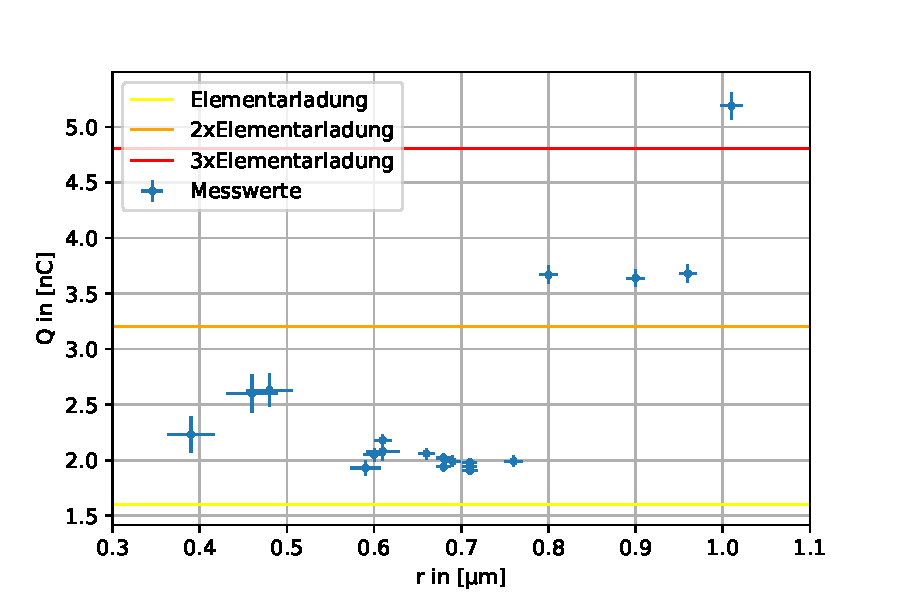
\includegraphics[width=1.0\textwidth]{QoverRUncorr.pdf}
		\caption{Ladung als Funktion des Radius}
	\end{figure}
	Es ist deutlich zu erkennen, dass eine Quantifizierung Wahrscheinlich ist, jedoch stimmt diese
	nicht mit den zu erwartenden Werten über ein, weswegen man die Cunningham Korrektur zu Hilfe nimmt.
	Mit der Cunningham Korrektur ergeben sich die Radien und Ladungen über
	\begin{equation}
		r_c = \sqrt{(\frac{A_c <l>}{2})^2 + r^2} - \frac{A_c <l>}{2}  
	\end{equation}
	\begin{equation}
		Q_c = Q(1+\frac{A_c<l>}{r_c})^{-1} \frac{r_c}{r}
	\end{equation}
	mit r als unkorrigierter Radius, $A_c=1.26$ als einheitenloser Faktor und $<l>=6.4\cdot 10^{-8} m$ als
	mitlere freie Weglänge eines Teilchens in Luft und den Fehlern
	\begin{equation}
		\Delta r_c = \frac{r \Delta r}{\sqrt{(\frac{A_c <l>}{2})^2 + r^2}}
	\end{equation}
	\begin{equation}
		\Delta Q_c = Q_c \sqrt{(\frac{\Delta Q}{Q})^2 + (\frac{A_c <l> \Delta r}{r(r+<l>A_c)})^2}
	\end{equation}
	Dies lässt sich erneut in folgender Tabelle darstellen und Plotten
	\begin{figure}[H]
		\begin{tabular}{c| c| c| c| c| c| c| c}
			\hline
			$r [\mu m]$ & $\Delta r [\mu m] $& $Q [10^{-9} C]$ & $\Delta Q [10^{-9} C]$ & $r_c [\mu m]$ & $\Delta r_c [\mu m]$ & $Q_c [10^{-9} C]$& $\Delta Q_c [10^{-9} C]$\\
			\hline
			0.61 & 0.019 & 2.1 & 0.08 & 0.57 & 0.019 & 1.7 & 0.08\\
			0.48 & 0.026 & 2.6 & 0.15 & 0.44 & 0.026 & 2.1 & 0.16\\
			0.71 & 0.008 & 1.9 & 0.04 & 0.67 & 0.008 & 1.7 & 0.04\\
			0.71 & 0.009 & 1.9 & 0.04 & 0.67 & 0.009 & 1.6 & 0.04\\
			0.66 & 0.008 & 2.1 & 0.05 & 0.62 & 0.009 & 1.7 & 0.05\\
			0.61 & 0.010 & 2.2 & 0.05 & 0.57 & 0.010 & 1.8 & 0.05\\
			0.90 & 0.010 & 3.6 & 0.08 & 0.86 & 0.010 & 3.2 & 0.08\\
			0.61 & 0.010 & 2.1 & 0.05 & 0.57 & 0.010 & 1.7 & 0.05\\
			0.46 & 0.030 & 2.6 & 0.17 & 0.42 & 0.029 & 2.0 & 0.18\\
			0.71 & 0.010 & 2.0 & 0.04 & 0.67 & 0.008 & 1.7 & 0.04\\
			0.80 & 0.010 & 2.0 & 0.04 & 0.64 & 0.008 & 1.6 & 0.04\\
			1.01 & 0.013 & 5.2 & 0.12 & 0.97 & 0.013 & 4.6 & 0.12\\
			0.60 & 0.012 & 2.0 & 0.06 & 0.56 & 0.012 & 1.7 & 0.06\\
			0.76 & 0.010 & 2.0 & 0.05 & 0.72 & 0.010 & 1.7 & 0.05\\
			0.68 & 0.010 & 2.0 & 0.04 & 0.64 & 0.008 & 1.7 & 0.05\\
			0.69 & 0.010 & 2.0 & 0.05 & 0.65 & 0.009 & 1.7 & 0.05\\
			0.80 & 0.010 & 3.7 & 0.08 & 0.76 & 0.010 & 3.2 & 0.08\\
			0.96 & 0.010 & 3.7 & 0.08 & 0.92 & 0.010 & 3.3 & 0.08\\
			0.58 & 0.017 & 1.9 & 0.07 & 0.54 & 0.017 & 1.6 & 0.07\\
			0.39 & 0.027 & 2.2 & 0.16 & 0.35 & 0.027 & 1.7 & 0.16\\
	   \end{tabular}
	\end{figure}		
	\begin{figure}[H]
		\centering
		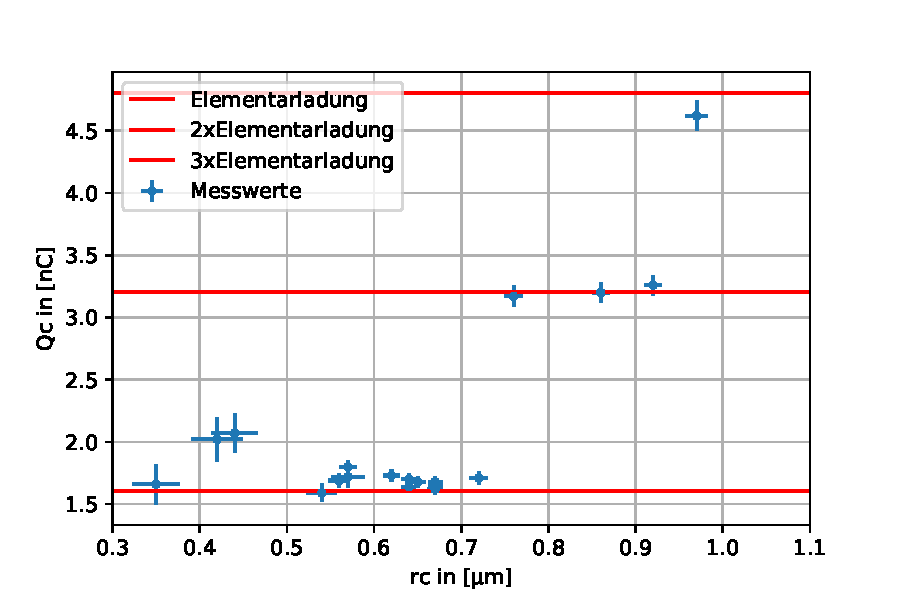
\includegraphics[width=1.0\textwidth]{QoverRUncorrCunt.pdf}
		\caption{$Q_c$ als Funktion von $r_c$}
	\end{figure}
	In dieser Grafik ist eine deutlich bessere Übereinstimmung der Messwerte mit der Quantisierten Elementarladung zu
	erkennen. Einige der Messwerte fallen leider nicht innerhalb des Fehlerbereichs mit einem Vielfachen der Elementarladung
	zusammen, diese Abweichung lässt sich für uns durch Ungenauigkeiten in der Messung zurückführen, wie zum beispiel
	die Umkehr der Kondersatorspannung und der daraus resultierenden kurzen Beschleunigungsstrecke, sowie die Bewegung der
	Teilchen in 3D, die Brownsche Molekularbewegung und die Umweltbedingte Bewegung der Luft im Kondensator.
	
	Zuletzt lässt sich nicht desto trotz die Elementarladung aus den Messwerten bestimmen. Dafür gilt
	\begin{equation}
		e = \frac{1}{\sum_{i=1}^n w_i} \sum_{i=1}^n Q_i \cdot w_i
	\end{equation}
	mit 
	\begin{equation}
		w_i = \frac{1}{\Delta Q_i^2}
	\end{equation}
	und dem Fehler
	\begin{equation}
		\Delta e = \sqrt{\sum_{i=1}^n\frac{1}{w_i}}
	\end{equation}
	Woraus sich für unsere Messung eine Elementarladung von $(1,83\pm 0.39)\cdot 10^{-19} C$ ergibt.
	Diese liegt innerhalb des Fehlerbereichs auf dem Literaturwert von $e=1.602176634\cdot 10^{-19}C$.
\section{Diskussion}
	Abschließend noch eine Zusammenfassung. Die unkorrigierten Messwerte stimmen, wie zu erwarten, 
	nicht mit den Literaturwerten über ein. Die korrigierten jedoch passen schon besser. 
	Auffällig ist, dass die korrigierten Ladungen und Radien geringer sind, als die ursprünglichen. 
	Dies war zu erwarten, da die Korrektur die Geschwindigkeiten nach unten korrigiert. 

	Der große Fehler bei unserem Ergebnis lässt sich dadurch erklären, dass bei der Berechnung
	der Elementarladung alle Messwerte eingeflossen sind. Bei Betrachtung der Grafiken wird jedoch deutlich,
	dass ein paar der Messwerte wahrscheinlich Mehrfachgeladen sind. Der Großteil ist aber Einfach geladen.
	Einige andere Fehlerquellen wären, wie oben schon kurz angeschnitten, dass die Teilchen auch einen Drift 
	aus der Bildebene raus hatten. Was dazu führt, dass die Tröpchen während des Messvorgangs größer/kleiner und
	bei einer zu späten Anpassung des Mikroskops unscharf wurden.

	Insgesamt hätte eine Statistik mit mehr Messwerten zu einem besseren Ergebnis geführt, da die Mehrfachladungen
	seltener sind, als die einfach geladenen Tröpchen. Jedoch ist auch unser Ergebnis mit 20 Tröpchen auf
	ein Ergebnis gekommen, welches mit Fehlerbereichs auf dem Literaturwert liegt.

\section{Anhang}
	%Fehlt: Tabelle für Messwerte
	\begin{figure}[H]
		\begin{tabular}{c|c|c|c|c|c|c|c}
			\hline
			$v_{sink} [\mu m/s]$ & $\Delta v_{sink} [\mu m/s]$ & $v_{steig} [\mu m/s]$ &$\Delta v_{steig} [\mu m/s]$ & $r [\mu m] $&$ \Delta r [\mu m]$ &$ Q [10^{-9} C] $&$ \Delta Q [10^{-9} C]$\\
			\hline
			213 & 5.5 & 122 & 1.8 & 0.61 & 0.019 & 2.1 & 0.08\\
			296 & 4.8 & 239 & 4.0 & 0.48 & 0.026 & 2.6 & 0.15\\
			196 & 2.1 & 70 & 0.9 & 0.71 & 0.008 & 1.9 & 0.04\\
			194 & 2.5 & 70 & 1.0 & 0.71 & 0.009 & 1.9 & 0.04\\
			207 & 2.3 & 100 & 1.1 & 0.66 & 0.009 & 2.1 & 0.05\\
			221 & 2.6 & 130 & 1.4 & 0.61 & 0.010 & 2.2 & 0.05\\
			298 & 3.4 & 98 & 1.6 & 0.90 & 0.010 & 3.6 & 0.08\\
			213 & 2.7 & 120 & 1.4 & 0.61 & 0.010 & 2.1 & 0.05\\
			304 & 5.5 & 253 & 3.6 & 0.46 & 0.029 & 2.6 & 0.17\\
			198 & 2.1 & 74 & 0.9 & 0.71 & 0.008 & 2.0 & 0.04\\
			197 & 2.1 & 81 & 0.9 & 0.68 & 0.008 & 1.9 & 0.04\\
			377 & 5.4 & 123 & 1.7 & 1.01 & 0.013 & 5.2 & 0.12\\
			212 & 2.6 & 124 & 2.1 & 0.60 & 0.012 & 2.0 & 0.06\\
			200 & 3.2 & 56 & 1.0 & 0.76 & 0.010 & 2.0 & 0.05\\
			203 & 2.2 & 89 & 1.0 & 0.68 & 0.008 & 2.0 & 0.04\\
			200 & 2.6 & 81 & 1.0 & 0.69 & 0.009 & 2.0 & 0.05\\
			303 & 3.4 & 144 & 1.7 & 0.80 & 0.010 & 3.7 & 0.08\\
			301 & 3.8 & 74 & 1.3 & 0.96 & 0.010 & 3.7 & 0.08\\
			204 & 3.9 & 120 & 3.0 & 0.58 & 0.017 & 1.9 & 0.07\\
			299 & 4.2 & 262 & 3.0 & 0.39 & 0.026 & 2.2 & 0.16\\
		\end{tabular}
		\caption{Tablle 1}
		\label{test}
	\end{figure}
\end{document}  